

\chapter{Shlukování}
\label{sec:shlukovani}

\par{V této kapitole bude popsáno učení bez učitele, algoritmus K-Means, cíl optimalizace, náhodná inicializace a volba počtu shluků.}









\section{Učení bez učitele}

\subsubsection*{Učení s učitelem}
\par{Typický problém učení s učitelem, kdy máme množinu vzorků $\bm{x}$ a k nim odpovídající informaci od učitele $y$. Trénovací množina má strukturu
\begin{equation}
	\left\lbrace \left( \bm{x}^{\left( 1 \right)} , y^{\left( 1 \right)} \right), \left( \bm{x}^{\left( 2 \right)} , y^{\left( 2 \right)} \right),  \left( \bm{x}^{\left( 3 \right)} , y^{\left( 3 \right)} \right), \ldots,  \left( \bm{x}^{\left( m \right)} , y^{\left( m \right)} \right) \right\rbrace .
\end{equation}
cílem je nalézt dělící nadrovinu, která bude nejlépe klasifikovat do dvou tříd.
\begin{figure}[!ht]
	\centering
	\begin{minipage}[t]{0.48\textwidth}
  		%trim option's parameter order: left bottom right top
		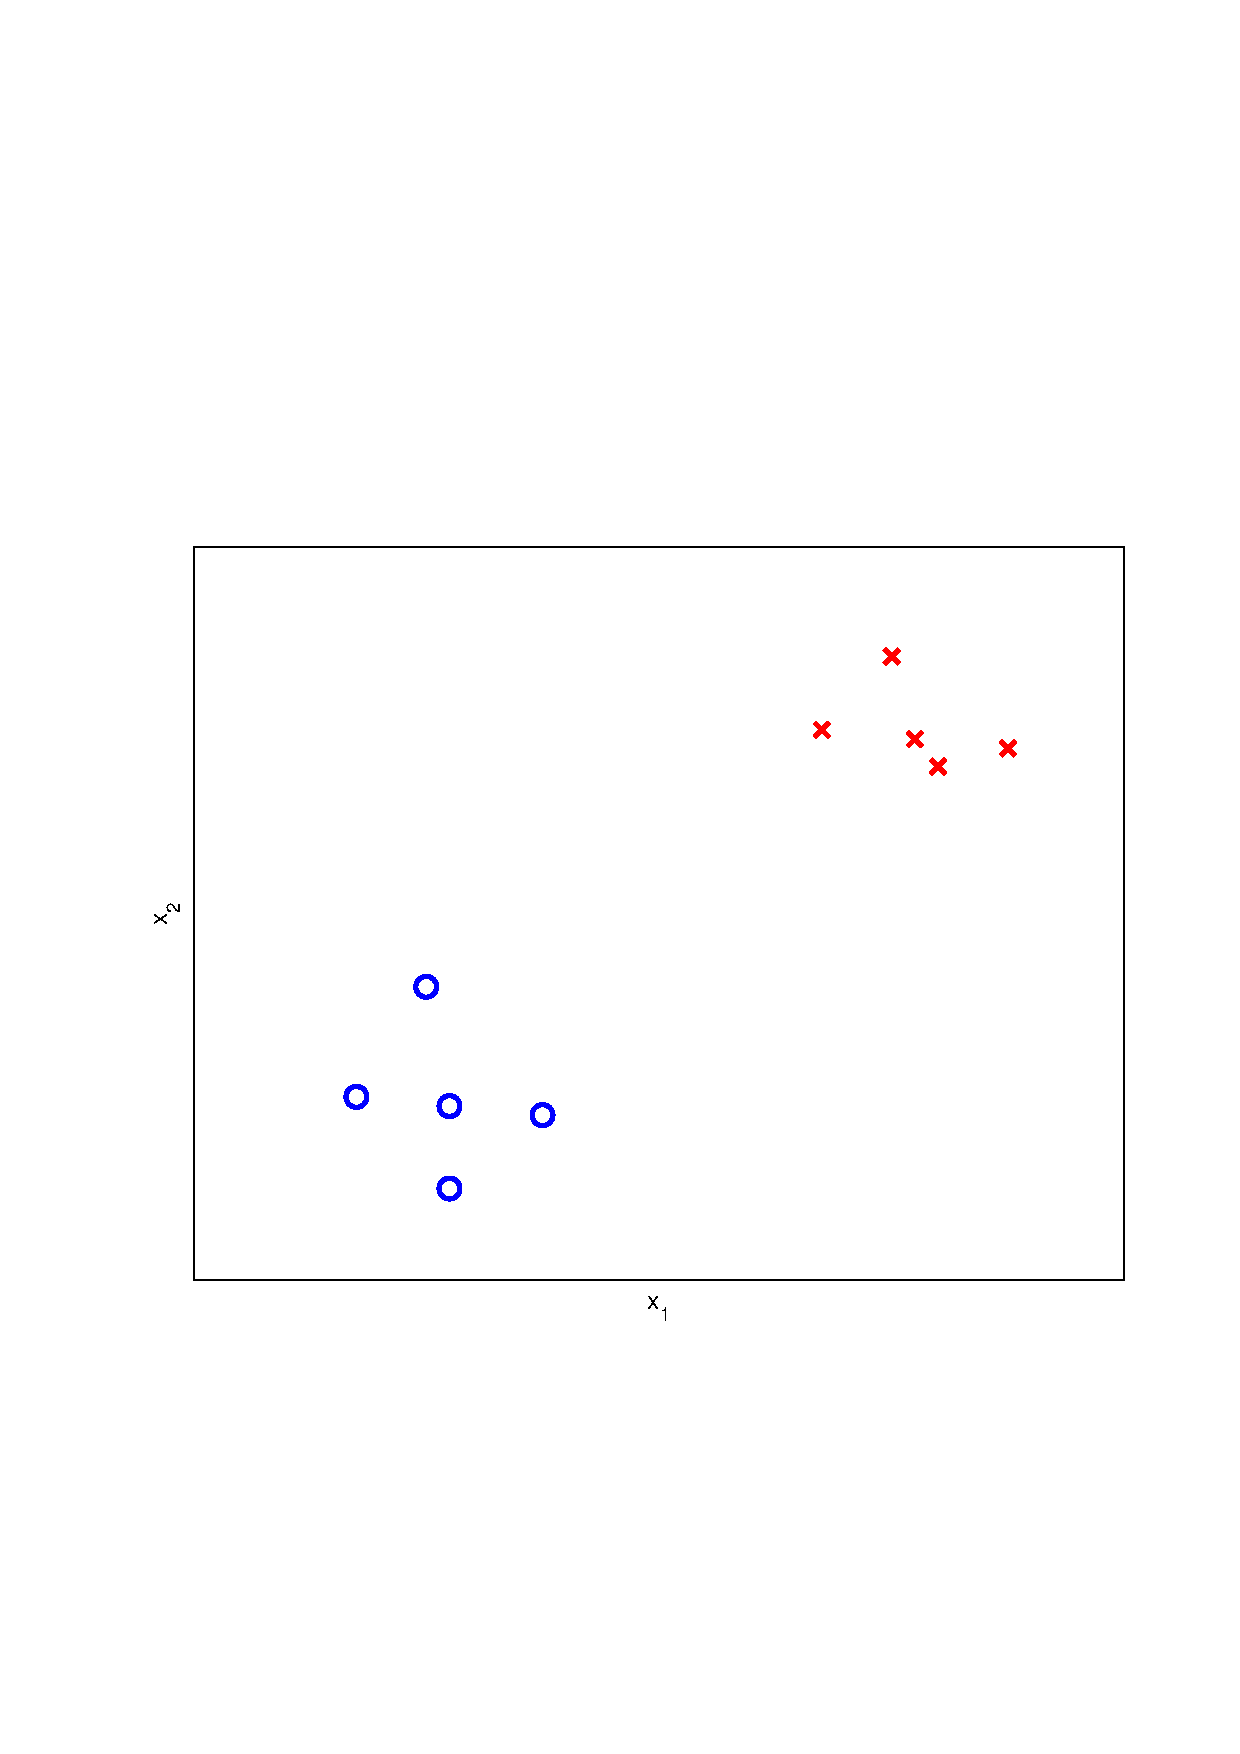
\includegraphics[width = \textwidth, trim = 2.5cm 7cm 2cm 9cm]{./Img/UnsupervizedLearning/Intro/supervized.pdf}
  		\caption{Klasifikace do dvou tříd - učení s učitelem.}
		\label{fig:supervized}
	\end{minipage}%
	\hfill
	\begin{minipage}[t]{0.48\textwidth}
		%trim option's parameter order: left bottom right top
		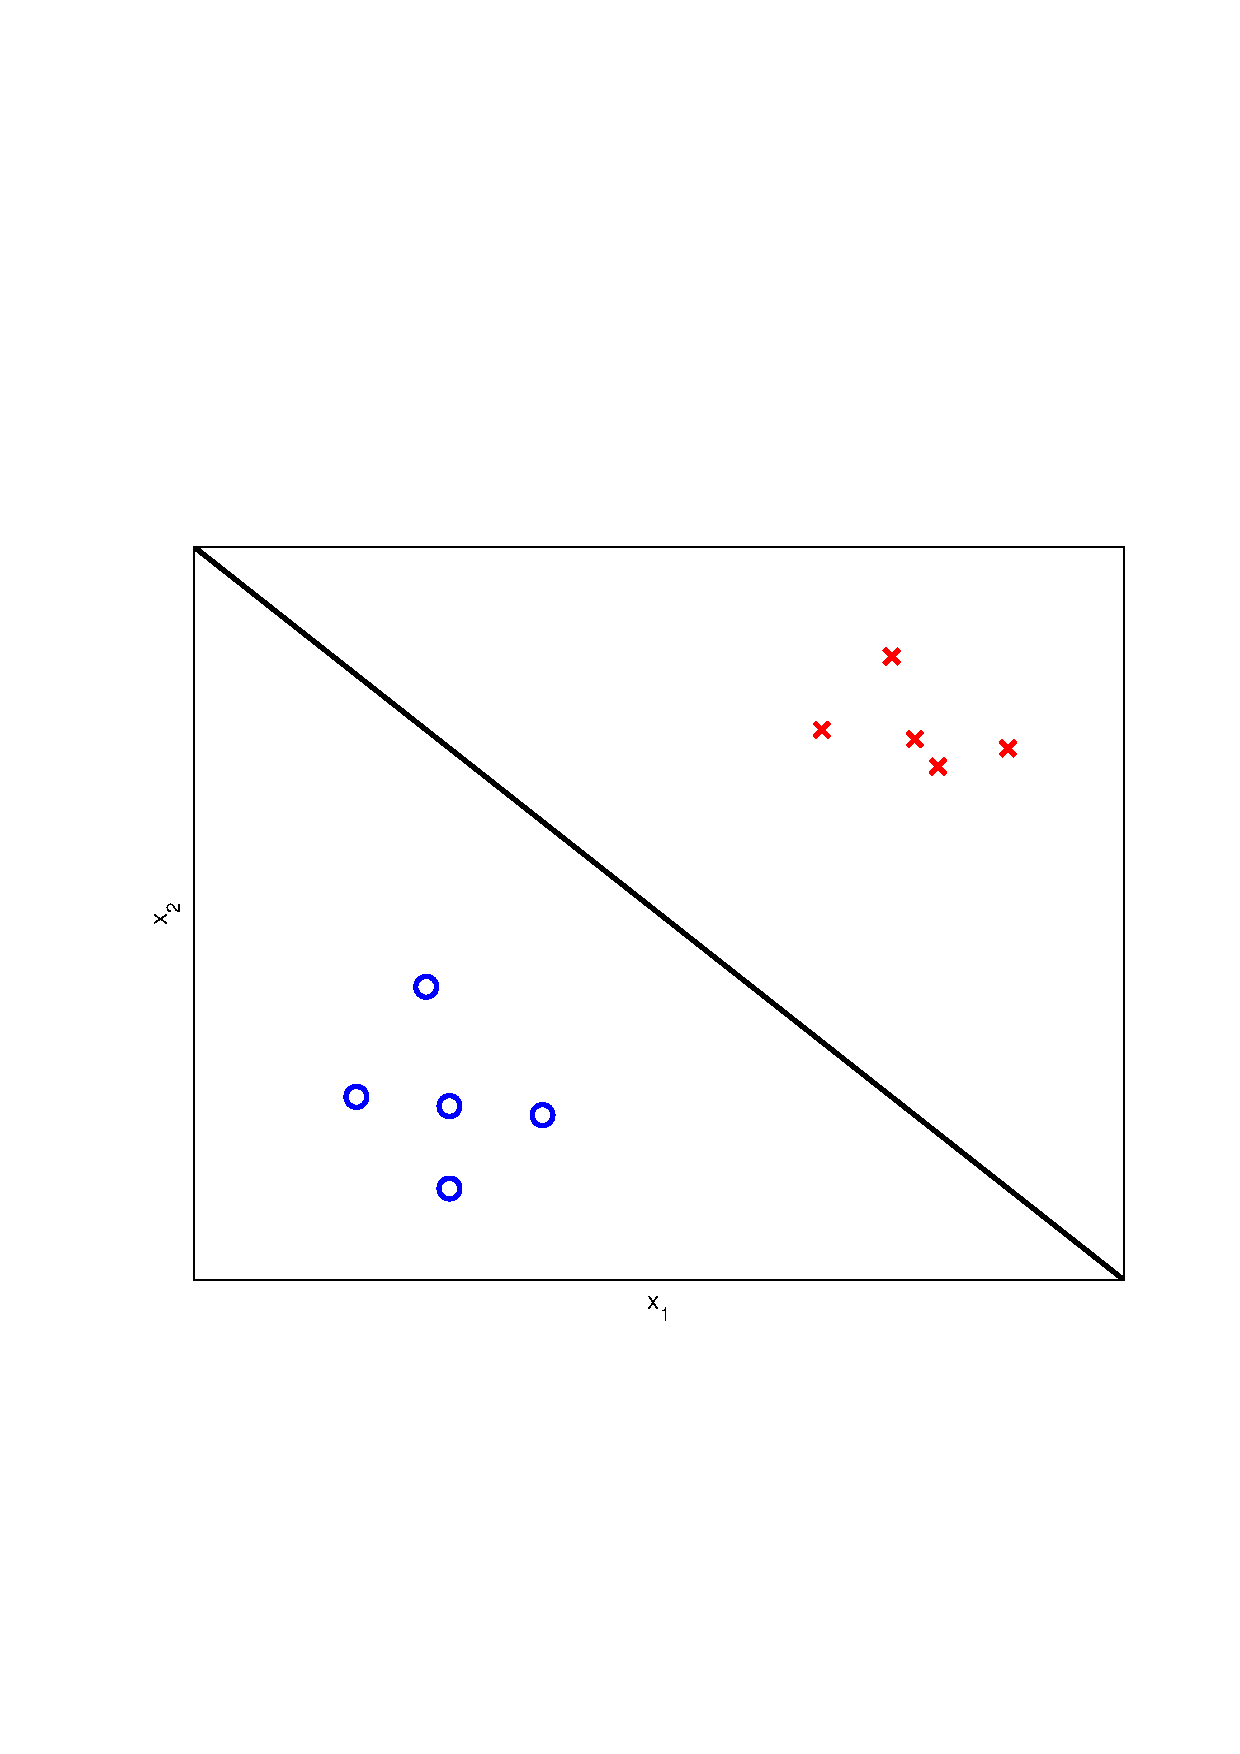
\includegraphics[width = \textwidth, trim = 2.5cm 7cm 2cm 9cm]{./Img/UnsupervizedLearning/Intro/supervized_line.pdf}
  		\caption{Klasifikace do dvou tříd s~dělící nadrovinou - učení s~učitelem.}
		\label{fig:supervized_line}
	\end{minipage}%
\end{figure}}

\par{Na Obr.~\ref{fig:supervized} a~\ref{fig:supervized_line} barva a~znak (kolečko nebo křížek) reprezentuje informaci od učitele.}

\newpage




\subsubsection*{Učení bez učitele}
\par{
V~případě učení bez učitele nemáme informaci od učitele do jaké třídy daný vzor patří. Trénovací množina má proto tvar
\begin{equation}
		\left\lbrace \bm{x}^{\left( 1 \right)} ,  \bm{x}^{\left( 2 \right)},   \bm{x}^{\left( 3 \right)} ,  \ldots,  \bm{x}^{\left( m \right)} \right\rbrace ,
\end{equation}
cílem učícího se algoritmu je nalézt strukturu mezi neznámými daty a~klasifikovat jednotlivé vzory do odpovídajících tříd. Je zřejmé, že v případě učení bez učitele postrádáme důležitou informaci o~počtu tříd. V~extrémních případech může být počet tříd roven jedné a~nebo počtu trénovacích vzorů. Na Obr.~\ref{fig:unsupervized}} a~\ref{fig:unsupervized_circle} lze vidět, že informace od učitele ve formě barvy a~znaku chybí.
\begin{figure}[!ht]
	\centering
	\begin{minipage}[t]{0.48\textwidth}
  		%trim option's parameter order: left bottom right top
		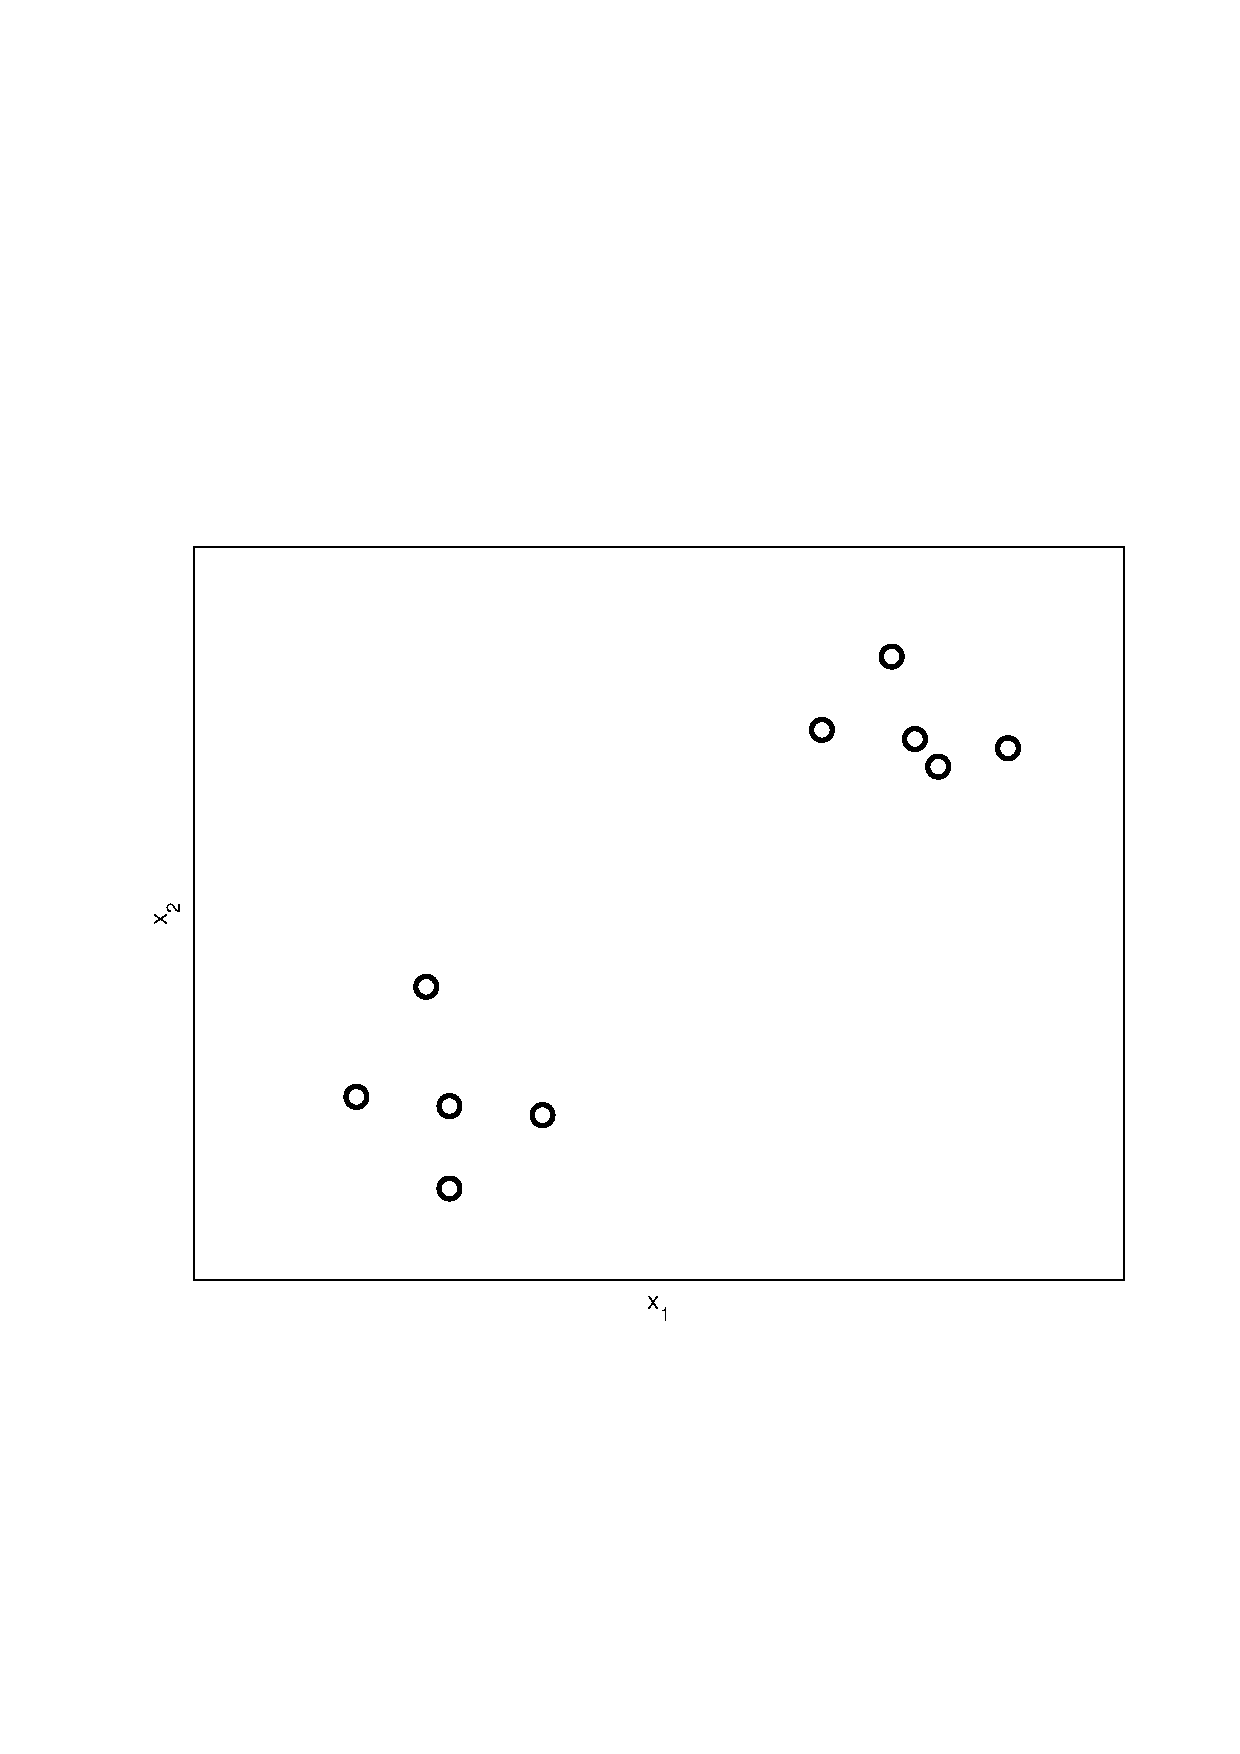
\includegraphics[width = \textwidth, trim = 2.5cm 7cm 2cm 9cm]{./Img/UnsupervizedLearning/Intro/unsupervized.pdf}
  		\caption{Klasifikace do dvou tříd - učení bez učitele.}
		\label{fig:unsupervized}
	\end{minipage}%
	\hfill
	\begin{minipage}[t]{0.48\textwidth}
		%trim option's parameter order: left bottom right top
		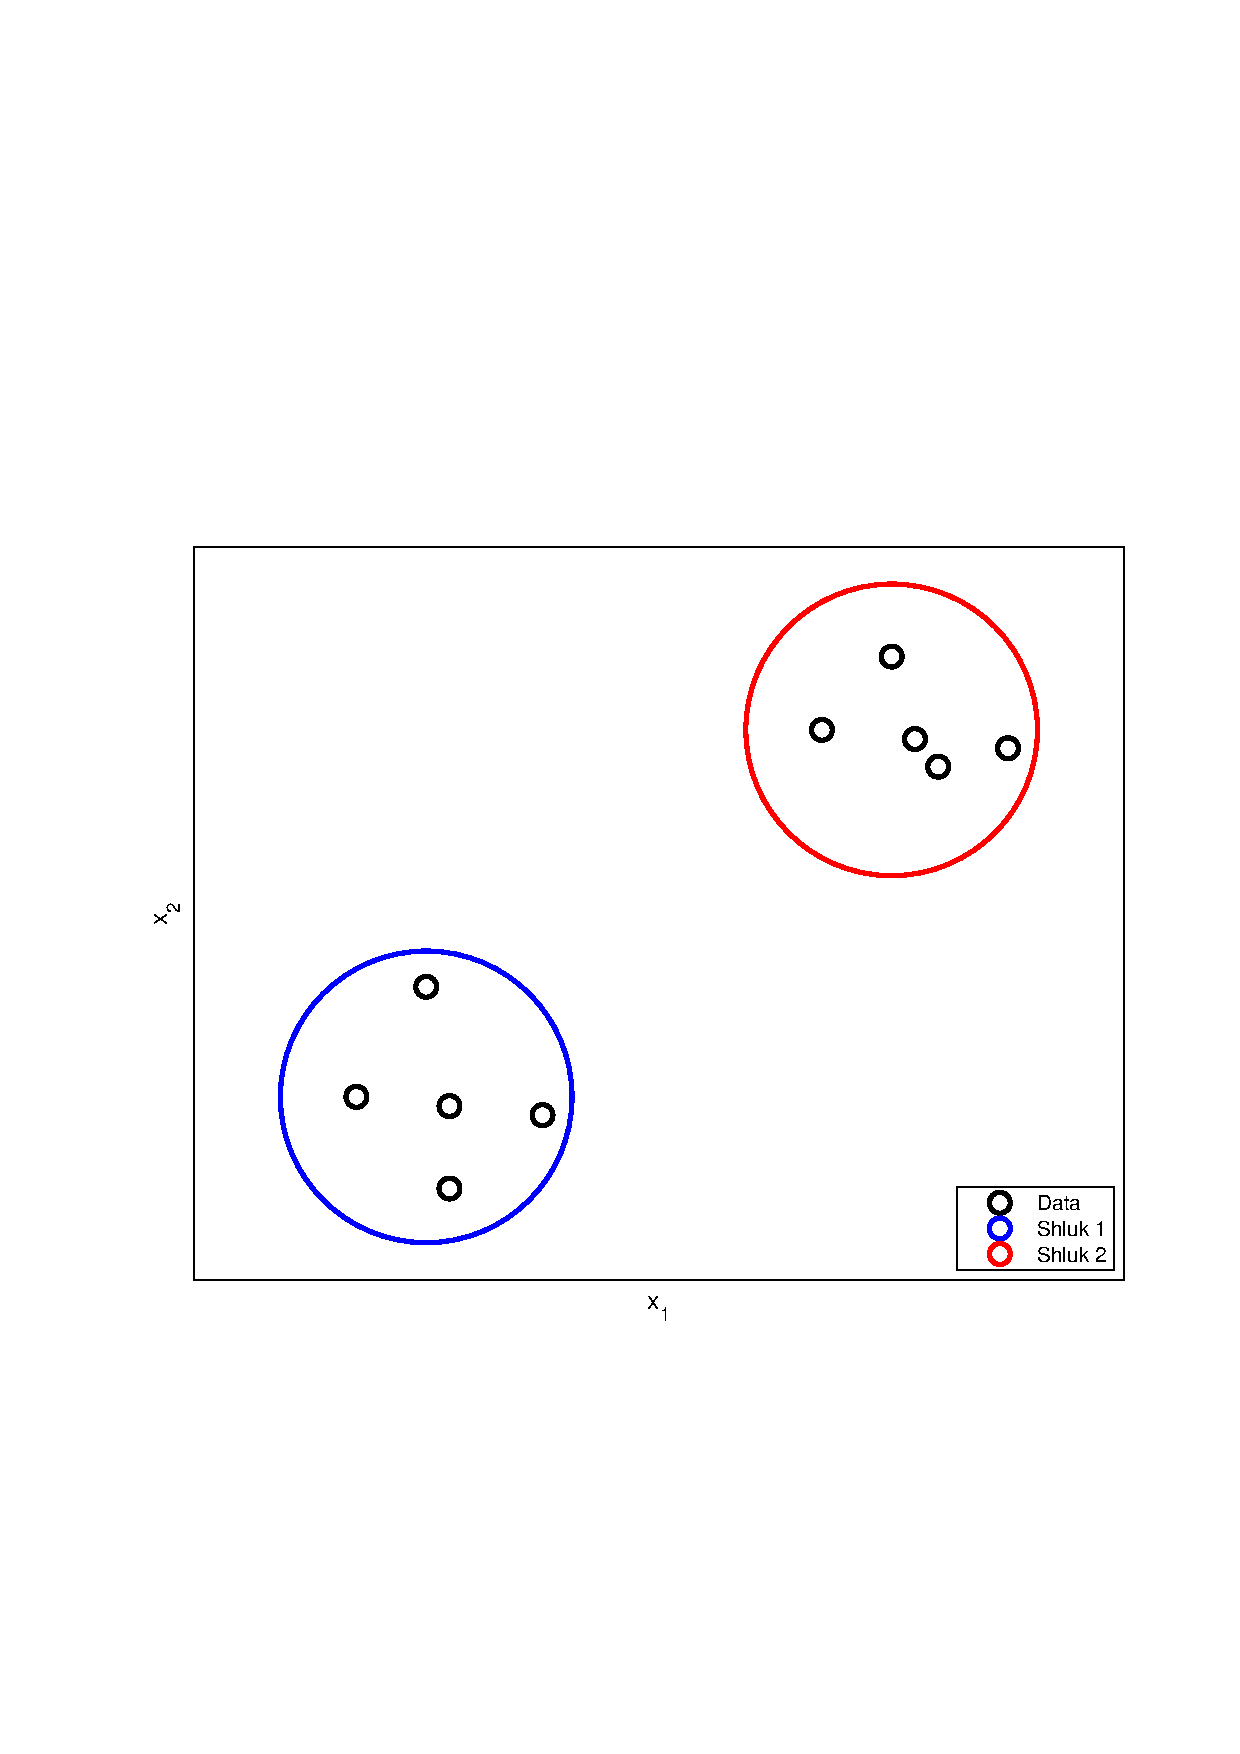
\includegraphics[width = \textwidth, trim = 2.5cm 7cm 2cm 9cm]{./Img/UnsupervizedLearning/Intro/unsupervized_circle.pdf}
  		\caption{Klasifikace do dvou tříd s naznačenými shluky - učení bez učitele.}
		\label{fig:unsupervized_circle}
	\end{minipage}%
\end{figure}}

\par{Příklad klasifikace v~případě učení bez učitele je \textbf{shlukování} , kde se jednotlivé třídy nazývají \textbf{shluky}.}



\newpage






\section{K-Means}

\par{}
\newpage











\section{Cíl optimalizace}

\par{}
\newpage











\section{Náhodná inicializace}

\par{}
\newpage











\section{Volba počtu shluků}

\par{}
\newpage
















